\chapter{Analisi dati}
Gli obiettivi principali di queste analisi sono:
\begin{itemize}
    \item Mostrare delle statistiche generali sul dust e sul comportamento degli indirizzi che lo ricevono;
    \item Descrivere alcuni pattern interessanti che sono stati trovati e che potrebbero rappresentare casi di Dust Attack.
\end{itemize}
\section{Statistiche generali}
I dati analizzati comprendono le transazioni dal \textbf{3 Gennaio 2009} al \textbf{10 Agosto 2017}.
Come spiegato precedentemento il primo obiettivo è quello di presentare statistiche generali sull'uso del dust, per questo motivo il primo compito eseguito è stato il filtraggio di tutte le transazioni dust. Le transazioni dust sono quelle transazioni che contengono almeno un input dust o almeno un output dust.
\begin{mdframed}
 infos:inputs:118890,\textbf{99},2;118902,9987098901,2 \checkmark\\
 infos:21482214,984902,114569039,1;21482868,\textbf{1},73028796,240:outputs \checkmark\\
 infos:118925,9963398109,121409,0:118926,9962398010,2 \textbf{x}
\end{mdframed}
Le prime due transazioni sono considerate nelle analisi successive, l'ultima invece è stata ignorata perchè di poco interesse ai fini dello studio del Dust Attack.\\
Le transazioni totali sono 245 410 083 mentre le transazioni dust sono 2 114 335, questo significa che il dust è presente solo nello 0.8\% delle transazioni totali; inoltre come riportato in\cite{dustAnalisi} 1 705 560 creano dust mentre solo 429 544 lo consumano. Da questi due ultimi risultati possiamo dedurre che ci sono transazioni in cui il dust è presente sia negli input che negli output.\\\\
Il passaggio successivo è stato il filtraggio delle transazioni generate da Satoshi Dice. Satoshi Dice\cite{SD} è un noto servizio di gambling, nato nell'Aprile 2012, che usa il dust per comunicare ai giocatori perdenti che hanno perso la loro scommessa. Data la notorietà del servizio, risulta molto poco probabile che l'intento sia quello di un Dust Attack.\\
Le transazioni generate da Satoshi Dice sono 1 465 295, ovvero il 69\% delle transazioni dust. Questo significa che i possibili attaccanti sono presenti nel rimanente 31\%, ovvero nelle restanti 649 040 transazioni dust.\\\\
Una volta ottenute tutte e sole le transazioni di interesse ho realizato i seguenti istogrammi che mostrano la distribuzione del numero di input dust e output dust. In entrambi i grafici le colonne rappresentano un gruppo di cinquanta valori.
\begin{figure}[h!]
    \centering
    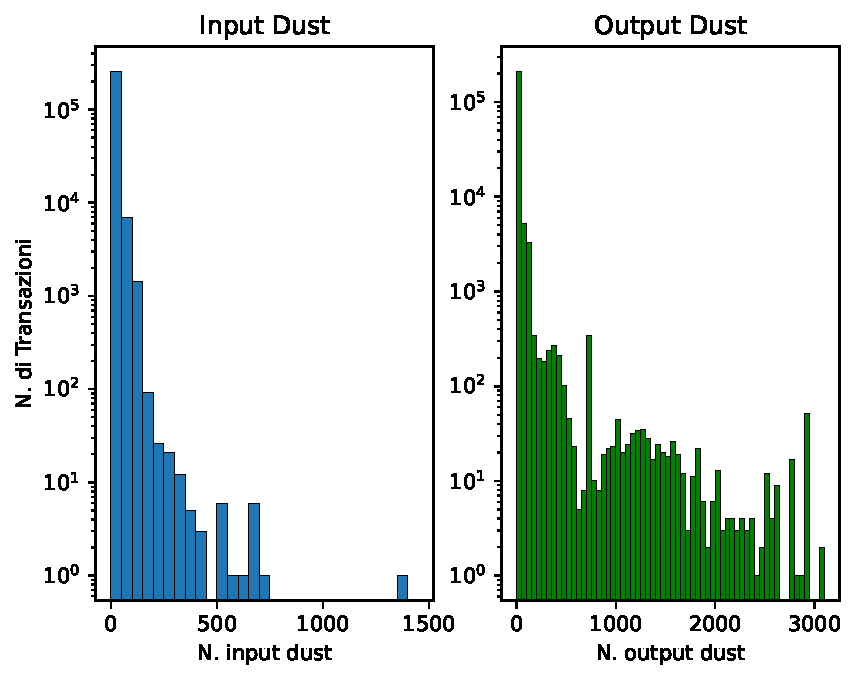
\includegraphics[scale=1]{Grafici/distribuzione_dust.pdf}
    \caption{Distribuzione numero input dust(sinistra) e output dust(destra)}
    \label{fig:dust_distribuzione}
\end{figure}
\FloatBarrier 
Dal primo istogramma possiamo notare come siano molto frequenti le transazioni con un numero di input dust nell'intervallo [1, 50), al contrario le transazioni con un elevato numero di input dust risultano poco usuali.\\
Il secondo grafico mostra come anche in questo caso sia molto frequente avere un numero di output dust nell'intervallo [1, 50). Al contratio del primo istogramma però possiamo notare come siano presenti molte più transazioni con un elevato numero di output dust. Da questi due grafici inoltre possiamo già intuire che molto output dust generato non venga successivamente speso.\\\\ 
Nelle analisi successive viene ignorato il dust generato con script OP\_RETURN. Questa scelta è motivata dal fatto che gli output con questo script non possono essere spesi; chi lo genera sicuramente non sta attuando un Dust Attack.\\
Il grafico seguente mostra la generazione del dust spendibile nel tempo.
\begin{figure}[h!]
    \centering
    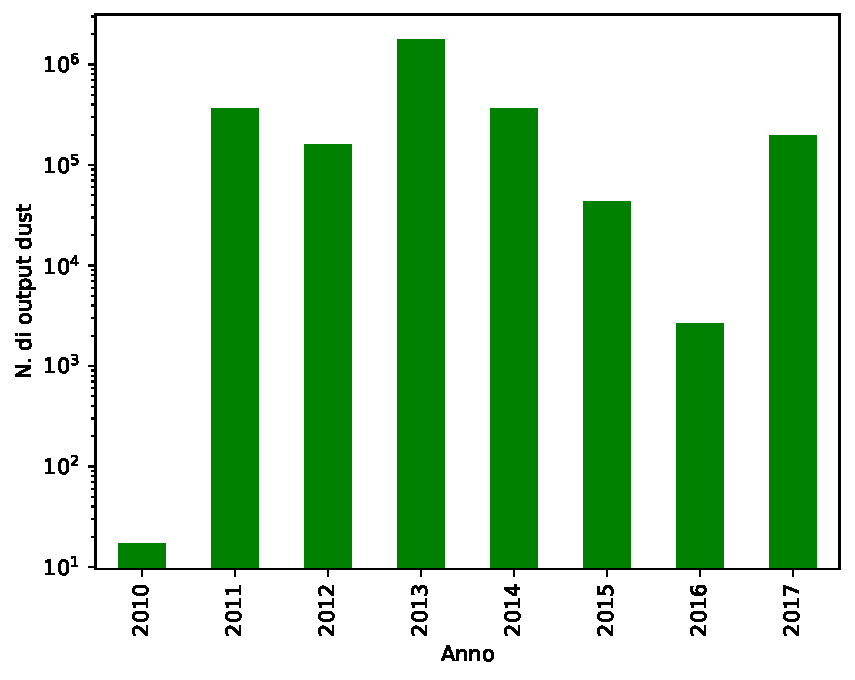
\includegraphics[scale=0.9]{Grafici/dust_created_year.pdf}
    \caption{Creazione dust nel tempo}
    \label{fig:dust_created}
\end{figure}
\FloatBarrier 
Dall'istogramma notiamo che già dal 2010 sono comparsi i primi output dust, anche se in quantità molto ridotta. Possiamo osservare una rapida salita tra il 2010 e il 2011, solo nel mese di luglio infatti sono stati generati 27 376 output dust tramite transazioni legate "a catena"; nel paragrafo successivo approfondirò il concetto delle "catene". 
Il picco della generazione di dust lo abbiamo nel 2013, dove sono state trovate diverse catene simili a quella del 2011 ma con una sostanziale differenza che spiegherò successivamente. Dopo il picco del 2013 osserviamo una diminuzione negli anni fino al 2017 dove sembrerebbe esserci una ricrescita. Bisogna però specificare che la maggior parte del dust generato nel 2017 proviene da due indirizzi: 1Enjoy1C4bYBr3tN4sMKxvvJDqG8NkdR4Z e 1SochiWwFFySPjQoi2biVftXn8NRPCSQC.\\Questi due noti indirizzi sono comparsi per la prima volta nel 2014 generando transazioni con circa 750 output di 1 satoshi ciascuno. La cosa interessante è che, nonostante il caos causato in vari forum Bitcoin, la tempesta di spam del 2014 "Enjoy Sochi" ha lasciato una piccola impronta sulla blockchain; solo 65 transazioni sono state confermate in quell'anno. L'aspetto singolare di questo fenomeno è che abbiamo visto echi di esso tornare negli anni successivi. Nel 2015 infatti sono state confermate 23 transazioni mentre nel 2017 sono presenti 255 transazioni generate da 1Sochi e 1Enjoy. Sebbene sia possibile che vengano eseguite dalla stessa entità, che spendeva importi da quegli indirizzi anche nel 2018, è anche possibile che qualcun altro abbia salvato le transazioni originali non confermate e le stia estraendo per qualche motivo. In questi tre anni il fenomeno "Enjoy Sochi" ha generato 343 transazioni per un totale di output dust intorno ai 255 000.\\\\
In generale sono stati generati 2 893 877 output dust con script diverso da OP\_RETURN; circa il 48.5\% è stato speso. Non è presente una grande differenza tra il dust non speso(51.5\%) e quello speso. Inoltre come possiamo osservare dalla tabella \ref{tab:dust_spent_unspent} la differenza è dovuta soprattutto agli anni 2011 e 2017; il dust del 2017 potrebbe essere stato speso successivamente. Dalla tabella inoltre notiamo la tendenza a spendere il dust nonostante possa provenire da indirizzi non noti come Satoshi Dice, quindi il prossimo obiettivo è capire come siano stati spesi questi importi.
\begin{table}[H]
    \centering
    \begin{tabular}{|c|c|c|c|c|c|c|c|c|}
        \hline
           categoria/anno   & 2010 & 2011 & 2012 & 2013 & 2014 & 2015 & 2016 & 2017\\
        \hline 
         speso &  3 & 825 & 55 352 & 601 685 & 303 484 & 392 823 & 28 026 & 20 695 \\
         \hline
         non-speso & 14 & 359 849 & 47 197 & 772 298 & 96 858 & 22 223 & 1272 & 191 273  \\
         \hline
    \end{tabular}
    \caption{Speso e Non-Speso negli anni}
    \label{tab:dust_spent_unspent}
\end{table}
Gli output dust spesi sono stati suddivisi in tre categorie:
\begin{enumerate}
    \item Successo: dust speso in transazioni che presentano almeno due indirizzi di input;
    \item Fallimento: dust speso in transazioni con un solo indirizzo di input;
    \item Speciale: dust speso in transazioni di "dust collecting".
\end{enumerate}
I termini "Successo" e "Fallimento" si riferiscono alla possibilità di collegare gli indirizzi di input una volta che il dust è stato speso. La terza categoria è stata separata dalla seconda prorpio per evidenziare l'uso del dust collecting.\\
Il grafico \ref{fig:dust_year} mostra quanto siano presenti le categorie nel corso degli anni.
\begin{figure}[h!]
    \centering
    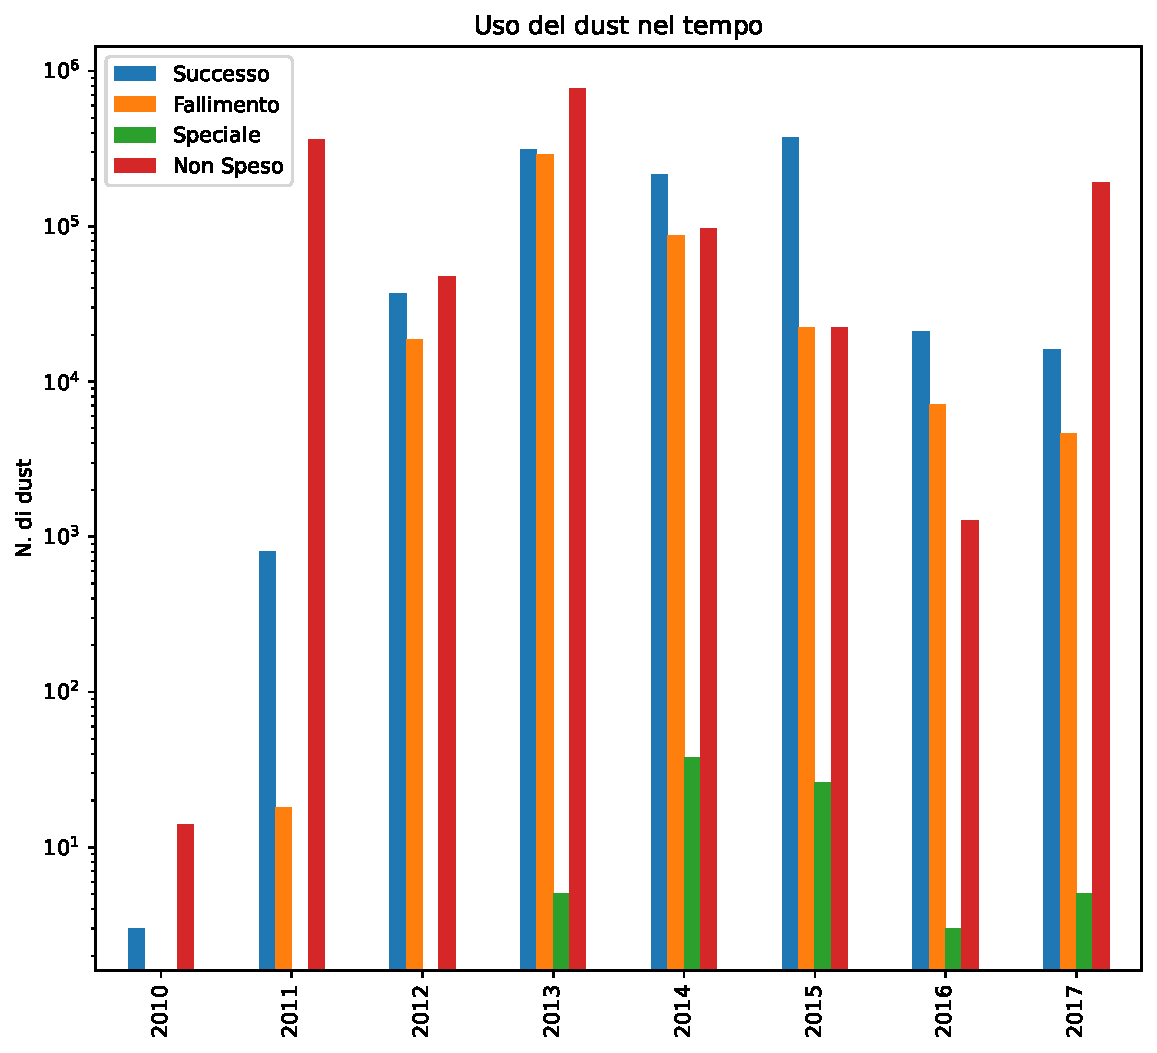
\includegraphics[scale=0.7]{Grafici/uso_del_dust_new.pdf}
    \caption{Uso del dust nel tempo}
    \label{fig:dust_year}
\end{figure}
\FloatBarrier
Non solo possiamo constatare graficamente quanto detto prima sulla differenza tra dust speso e non speso, ma possiamo anche trarre due importanti riflessioni. La prima riguarda l'uso del "dust collecting", risulta evidente quanto poco sia stato utilizzato questo servizio. La seconda invece riguarda la tendenza a spendere il dust con almeno un altro indirizzo, in particolare notiamo un netto distacco nel 2015 dove la categoria "Successo" rientra nell'ordine di $10^4$ mentre "Fallimento" nell'ordine di $10^3$. Gli indirizzi che hanno generato il dust potrebbero aver avuto altre motivazioni diverse dal Dust Attack, in molti casi però sono riusciti a ottenere lo stesso risultato, ovvero collegare più indirizzi tra loro.\\\\
Una volta constatata la presenza di transazioni con input dust e con almeno due indirizzi diversi, la fase seguente è l'analisi delle transazioni. Abbiamo tre categorie di transazioni: almeno due indirizzi diversi, un solo indirizzo e dust collecting.\\
In totale il dust è stato speso in 263 963 transazioni, la tabella \ref{tab:tx_categories} mostra il numero totale di transazioni nelle tre categorie, la tabella \ref{tab:tx_categories_year} mostra una visione annuale.
\begin{table}[H]
    \centering
    \begin{tabular}{|c|c|}
        \hline
        2+ indirizzi & 166 906\\
        \hline
        1 indirizzo & 97 040\\
        \hline
        dust collecting & 17\\
        \hline
    \end{tabular}
    \caption{Transazioni nelle tre categorie}
    \label{tab:tx_categories}
\end{table}
\begin{table}[H]
    \centering
    \begin{tabular}{|c|c|c|c|c|c|c|c|c|}
        \hline
            categoria/anno  & 2010 & 2011 & 2012 & 2013 & 2014 & 2015 & 2016 & 2017\\
        \hline 
         2+ indirizzi &  3 & 206 & 6741 & 82 702 & 49 499 & 20 155 & 3476 & 4124 \\
         \hline
         1 indirizzo & 0 & 16 & 5390 & 38 199 & 38 919 & 11 095 & 2066 & 1355  \\
         \hline
         dust collecting & 0 & 0 & 0 & 3 & 6 & 5 & 2 & 1 \\
         \hline
    \end{tabular}
    \caption{Transazioni nel tempo}
    \label{tab:tx_categories_year}
\end{table}
Dalle tabelle \ref{tab:tx_categories} \ref{tab:tx_categories_year} confermiamo quanto detto prima, la prevalenza a spendere il dust in transazioni con almeno due indirizzi diversi e lo scarso utilizzo di servizi come Dust-B-Gone; la seconda fase delle analisi si concentrerà sui primi due gruppi.\\
La categoria "1 indirizzo" è stata ulteriormente suddivisa in due classi:
\begin{itemize}
    \item NOD: transazioni che presentanto input con importo $>$ 545  
    \item OD: transazioni con soli input dust.
\end{itemize}
Dalla tabella \ref{tab:OD_NOD} possiamo dedurre che il fallimento nella de-anonimizzazione sia dovuto principalmente a quegli indirizzi che non sono vuoti, ovvero hanno ricevuto importi non-dust da altre fonti. 
\begin{table}[H]
    \centering
    \begin{tabular}{|c|c|c|}
        \hline
            NOD  & 92 712 & 95,5\%\\
        \hline 
            OD  & 4328 & 4,5 \%\\
        \hline
    \end{tabular}
    \caption{Classificazione OD e NOD}
    \label{tab:OD_NOD_failed}
\end{table}
Interessante invece è il secondo gruppo, in particolare due indirizzi: 1JwSSubhmg6iPtRjtyqhUYYH7bZg3Lfy1T e 1PEDJAibfNetJzM289oXsW1qLAgjYDjLgN. Il fatto interessante del primo indirizzo è che che la sua chiave privata è stata compromessa\footnote{fonte:\url{https://privatekeys.pw/address/bitcoin/1JwSSubhmg6iPtRjtyqhUYYH7bZg3Lfy1T}}, questo consente a chiunque di riscattare bitcoin non appena gli vengono inviati.\\\\
Caso anomalo invece riguarda 1PEDJAibfNetJzM289oXsW1qLAgjYDjLgN, rinominato 1PED per semplicità. Questo indirizzo, come riportato in\cite{dustAnalisi} è un noto gambler di Satoshi Dice, la singolarità però deriva da alcune transazioni che ha generato. In queste transazioni infatti è presente un solo input di 1 satoshi e un solo output, ovviamente sempre di 1 satoshi. Questi singoli satoshi però non provengono da Satoshi Dice ma da altri indirizzi che seguono un pattern ben preciso, schematizzato nella figura \ref{fig:1PED}
\begin{figure}[h!]
    \centering
    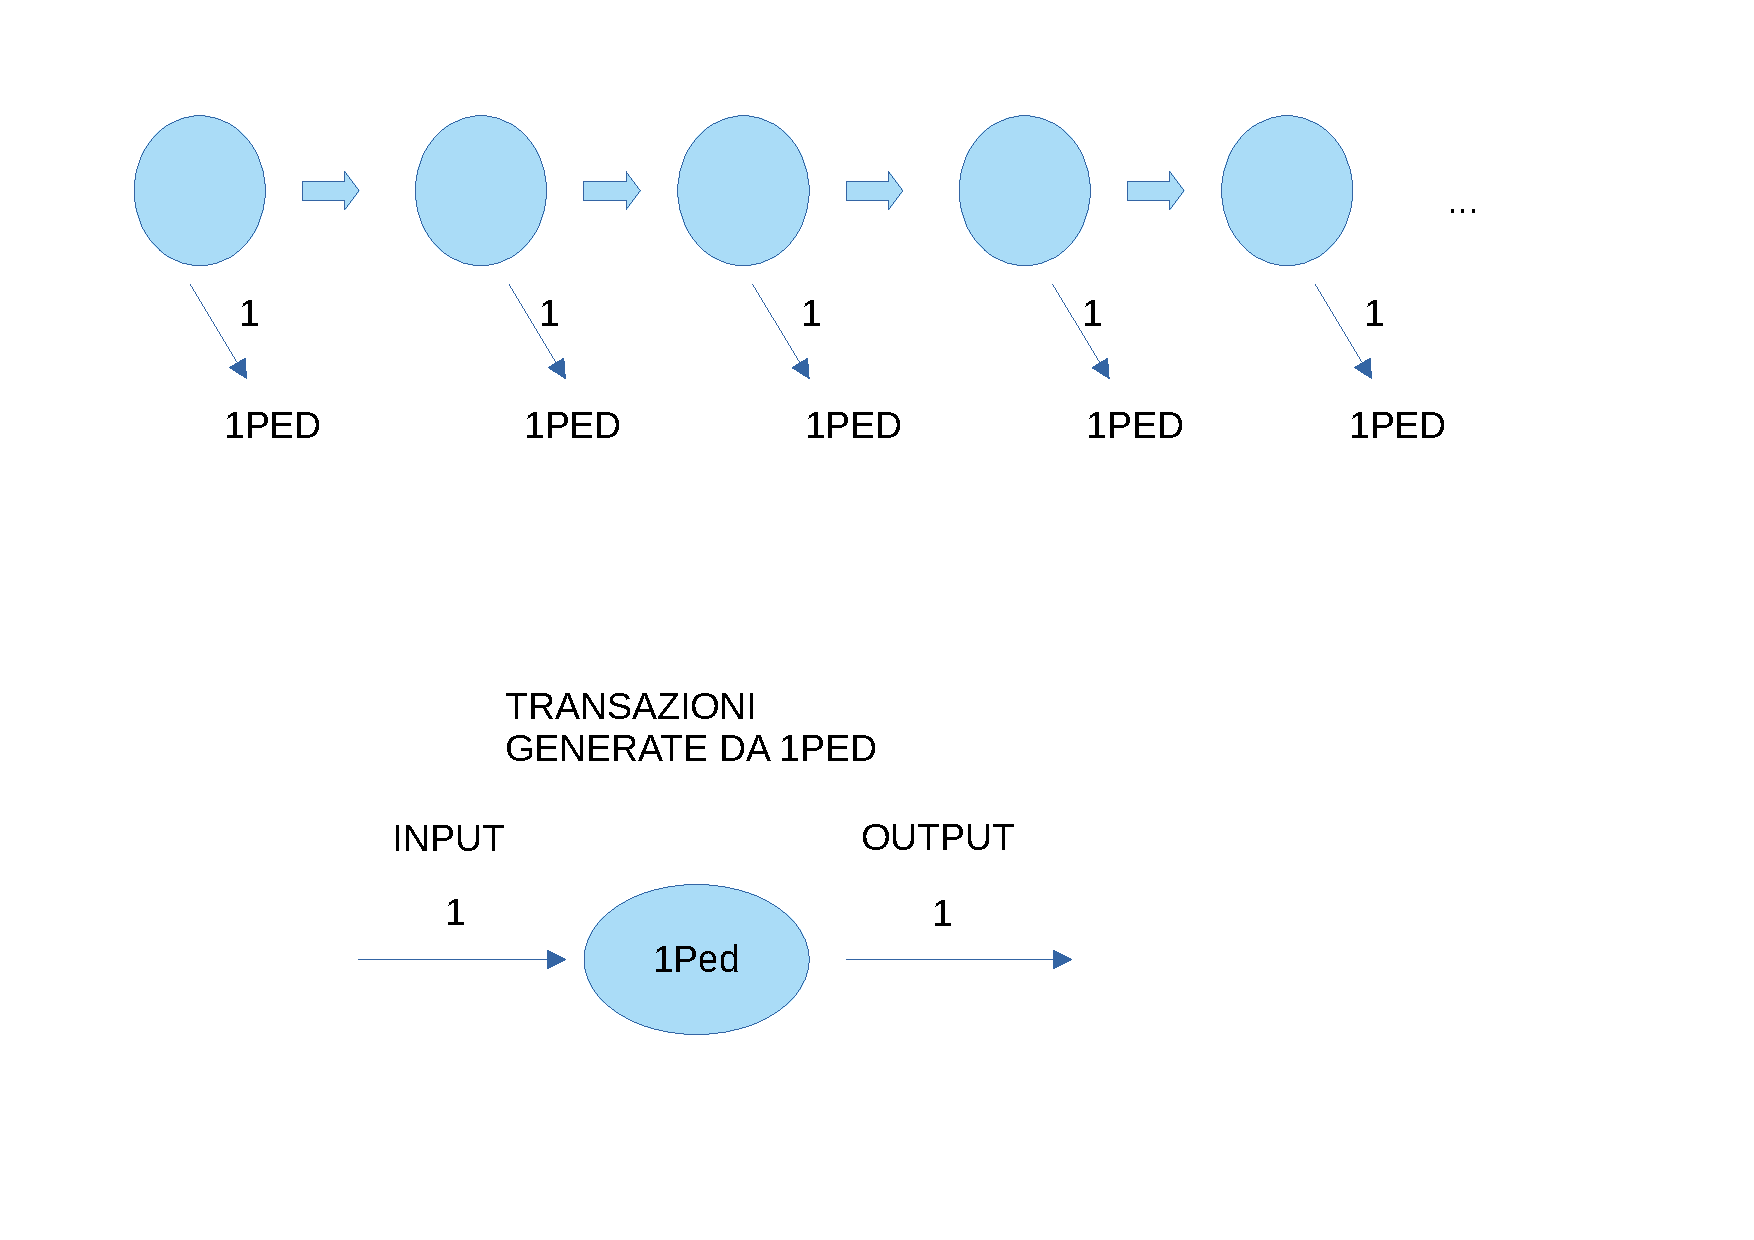
\includegraphics[scale=0.4]{Images/1Ped.pdf}
    \caption{Schema transazioni legate a 1PED}
    \label{fig:1PED}
\end{figure}
\FloatBarrier
Ogni indirizzo invia due output, 1 satoshi con destinatario 1PED e un secondo importo che viene inviato ad un altro indirizzo che seguirà il medesimo schema; in tutte queste transazioni la fee è di 50 000 satoshi. 1PED ha generato poi 1835 transazioni con 1 solo satoshi di input e 1 solo satoshi di output, la data è il 10 Marzo 2013 alle ore 16:20. Gli indirizzi destinatari però compaiono nella blockchain per la prima volta proprio grazie a queste transazioni, sicuramente non si tratta di un tentativo di Dust Attack.\\\\
Molto più interessanti sono le transazioni della categoria "2+ indirizzi". Anche in questo caso vengono mostrati i gruppi OD e NOD. La tabella \ref{tab:OD_NOD_success} mostra come quasi sempre si riescano a collegare indirizzi vittima di dust con indirizzi più capienti.
\begin{table}[H]
    \centering
    \begin{tabular}{|c|c|c|}
        \hline
            NOD  & 166 778 & 99,9\%\\
        \hline 
            OD  & 128 & 0,1 \%\\
        \hline
    \end{tabular}
    \caption{Classificazione OD e NOD}
    \label{tab:OD_NOD_success}
\end{table}
È importante però capire quanto successo abbia avuto la de-anonimizzazione in generale e negli anni. La tabella \ref{tab:stat} mostra alcune statistiche generali mentre la tabella \ref{tab:stat_year} fornisce una visione annuale.
\begin{table}[H]
    \centering
    \begin{tabular}{|c|c|}
        \hline
            Media Numero Input & 27\\
        \hline 
            Moda numero di input & 4\\
        \hline
            Percentuale media numero input non-dust & 71 \%\\
        \hline
            ercentuale media numero input dust & 29 \%\\
        \hline
            Media numero indirizzi diversi & 13\\
        \hline
            Moda numero indirizzi diversi & 2\\
        \hline
    \end{tabular}
    \caption{Statistiche generali}
    \label{tab:stat}
\end{table}
\section{Pattern Particolari}
\begin{itemize}
    \item catena dust
    \item tante Tx stesso timestamp stesso tutto
    \item tante Tx breve tempo, tanti output ecc...
\end{itemize}